\chapter{Compiler} \label{sec:compiler}

In this section, we introduce the compiler framework---\name---that targets Plasticine
architecture from high-level programs described in the Spatial language. 

\paragraph{Front-end Selection} 

\begin{figure*}
\centering
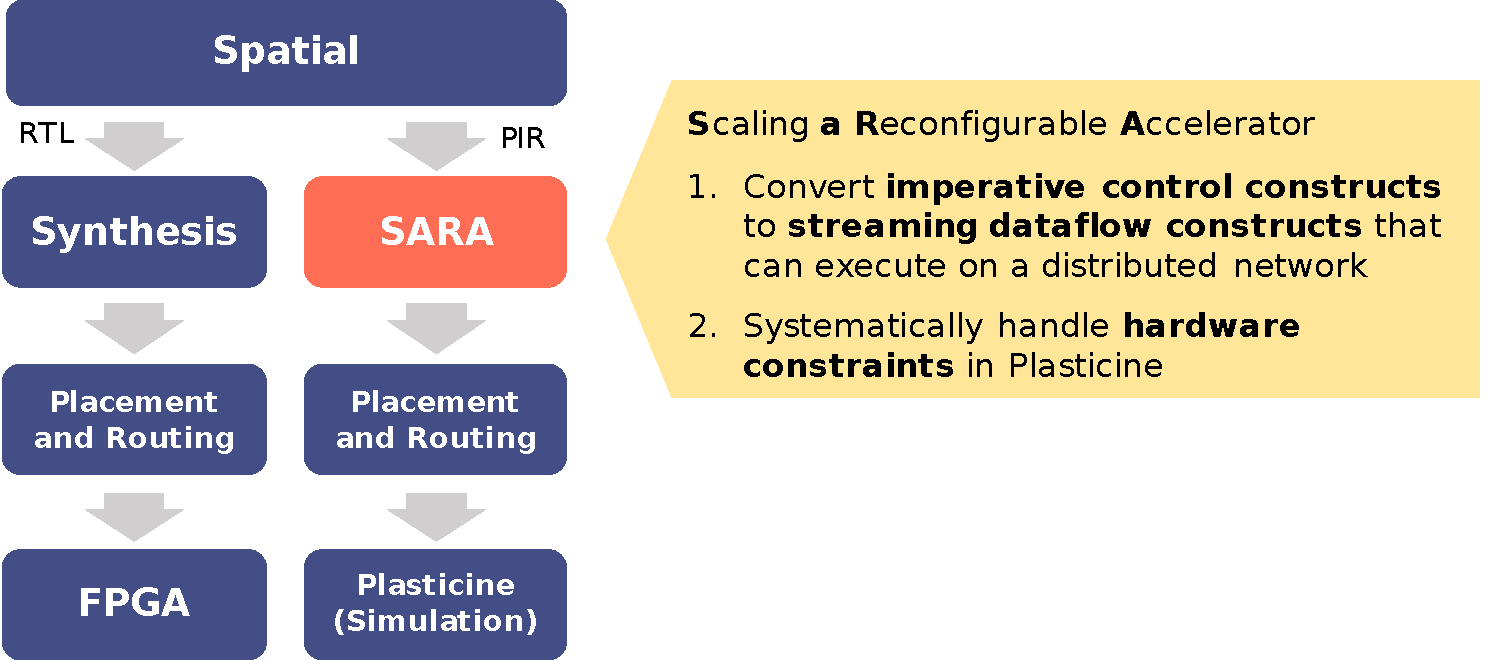
\includegraphics[width=1\textwidth]{figs/spatialstack.pdf}
\caption[Spatial Stack]{Spatial Stack}
\label{fig:spatialstack}
\end{figure*}

Although \name takes Spatial as front-end, the compilation techniques in \name can be equally
applied to other imperative langauges with nested loop constructs, such as C-based high-level
syntehsis language, the backend of Halide IR, and other DSLs at the similar abstraction level. 
Using Spatial as our front-end language has the advantage that the language is designed for
reconfigurable hardware, such that it can express valid execution schedule that can be exploit by
spatial architectures natively in the language.

%% Memory model
The data structure reprsented most exisitng imperative languages IR often marries to the
CPU's virtual memory model. LLVM-based compilers, for example, treats data collections as pointers to a shared
global address space, without distinguising what data are stored on-chip vs. off-chip.
This is CPU provides the memory abstraction that any data within the global address space 
can be equally accessed and the hardware implicitly manage the data movement between on and off-chip 
access by brining
Accelerators on the other hand, has explicitly managed on-chip scratchpads, that is not a cached
version of main memory data implicitly managed by the hardware.
The idea is to have the algorithm, which has better understanding of the data characteristics, to
explicitly control what data gets moved on and off-chip to maximize locality.
Other important static analysis in synthesis compilers, such as banking analysis, requires the
compiler to have the global view all access patterns on a data structure.
Therefore, modeling the data structures as disjoint memory space is much more suitable 
than pointers to a shared memory for reconfigurable architectures.

Spatial currently does not capture procedure calls in the IR; all functions are inlined and does not
share resources. A future work is to use synchronization mechanism in \name to implement true procedure
call on a spatial architecture.

Without lost of generality, we use python-style pseudo code to represents the front-end programming
abstraction the the rest of our discussion.

\section{Native Low-level Programming Interface of Plasticine}
Similar to FPGA high-level synthesis tools, \name provides a high-level imperative programming
abstraction and synthesizes the program to execute on a reconfigurable accelerator. Targeting an \rda, however,
is much more challenging than targeting FPAGs due to \rda's stringent mapping constraints. 
Unlike FPGAs, \rdas cannot map arbitrary RTL functionality. 

Taking Plasticine as an example, 
the hardware has collection of memory tiles (PMUs) and compute tiles (PCUs). 
The mesh global network can be statically configured to connect any tiles with guaranteed in-order 
transmission of packets over arbitrary network latency.

\subsubsection{Pattern Compute Unit (PCU)}
As the major compute work horse of the architecture, a PCU contains a 6-stage SIMD pipeline with 16 SIMD lanes. 
Unlike a processor core, the PCU can only statically configure six vector instructions throughout the
entire execution.
Additionally, the six instructions must be branch-free in order to be fully pipelined across stages.
At runtime, the SIMD pipeline executes the same set of instructions over different input data.
Software can configure the SIMD pipeline to depend on a set of input streams and
produce a set of output streams. 
There are three types of streams--single-bit control streams, 32-bit word scalar streams, and
16-word vector streams--corresponding to three types of global networks.
Execution of the PCU is triggered by the arrival of its input dependencies and back pressured by
the downstream buffers.
The PCU also contains configurable counters, which can be chained to produce the values of nested
loop iterators used in the datapath. 

\begin{figure}
\inputminted{python}{code/context.py}
\caption[Example context configuration]{Simplified pseudo context configuration}
\label{fig:context}
\end{figure}

We refer to the program graph that can be executed by the SIMD pipeline as a \term{compute context} or
simply \term{context}. 
A context includes the branch-free instructions mapped across SIMD stages, the input and output 
streams, and associated counter states and control configurations.
\Cref{fig:context} shows example of simplified pseudo assembly code to program a PCU context.
The control signals of the configurable counters, such as counter saturation or \term{counter done}
signals, can be used to dequeue and enqueue the input and output streams, respectively.
The counter bounds (i.e. min, max, and stride) can also be data-dependent using values from the 
scalar input streams. Compared to other data-flow architectures, the data-flow engine in Plasticine 
is more flexible in that it allows dynamic enqueue and dequeue window for its input and output streams.
\emph{This feature enable Plasticine to support complex control hierarchy, such as nested loops and
branch statements, across contexts even though individual contexts can only executes instructions that are
control-free}. 

There is no global scheduler to orchestrate the execution order among contexts---the execution is purely
streaming and data-flow driven. 
The only way to order the execution of two contexts without a data-dependency is to 
introduce a control \term{token} between two contexts acting like a dummy data-dependency.
This restriction eliminates the need of long-travelling wires and communication hot spot caused by a
centralized scheduler, which  again improves the clock frequency and scalability of the architecture.

\subsubsection{Pattern Memory Unit (PMU)}
PMUs hold all distributed scratchpads available on-chip. 
Each PMU contains 16 SRAM banks with
32-word access granularity. The PMU also contains pipeline stages specialized for address
computation. Unlike SIMD pipelines in PCUs, these pipeline stages are non-vectorized and can only 
perform integer arithmetics. 
The address produced by the address pipeline is broadcasted to 16 banks with a configurable offset added to each bank.
In contrast to PCU SIMD pipeline that has to be programmed atomically, the address pipeline stages 
within PMUs can be sliced into a write and a read context, triggered independently.
In addition to compute stages, resources such as I/O ports, buffers, and counters are also shared across contexts.
It is the software's responsibility to make sure total resources consumed by all
contexts does not exceed resource limits of the PMU.
All contexts within PMU have access to the scratchpads with unprotected order. For instance, to
restrict a read context to access the scratchpad after the write context, the software must explicitly allocate
a token from the write context to the read context.
\name automatically generates required control tokens across context such that the memory access order is
consistent to the one from high-level program order.

Unlike most accelerators at this scale, Plasticine does not have any shared global on-chip memory. 
This design dramatically improve the memory density and scalability of the architecture 
by eliminating hardware complexity and overhead to support complex cache coherence protocol.
%% TODO: add a sentence commenting on the network bandwidth
On the other hand, however, the burden of maintaining consistent view of a logical memory mapped
across distributed scratchpads is left to the software.
The software must explicitly configure synchronizations across PCUs and PMUs, taking into account
that the network can introduce variable latency on both control and data path.
One of the major contribution of \name is to hide these synchronization burden from the programmer
and still provide a programming abstraction of logical memories with variable bandwidth and 
arbitrary capacity that fits on-chip.

\subsubsection{DRAM Interface}
The Plasticine architecture provides access to four DDR channels on the two sides of the
unit array. Each side has a column of DRAM address generator (DAG) specialized to generate off-chip
requests. Like compute pipeline in PMUs, the pipeline in DAG is also non-vectorized with integer
arithmetics. Each DAG can generates a load or a store request streams to the off-chip memory. All
streams can access the entire address space of the DRAM, with in-order response within each stream
and no ordering guaranteed across streams. To provide off-chip memory consistency, \name allocates
synchronizations across request generator and response receiver contexts to preserve memory ordering
specified in the program.

\subsubsection{Abstract Programming Model}

\section{Compiler Overview}

\begin{figure*}
\centering
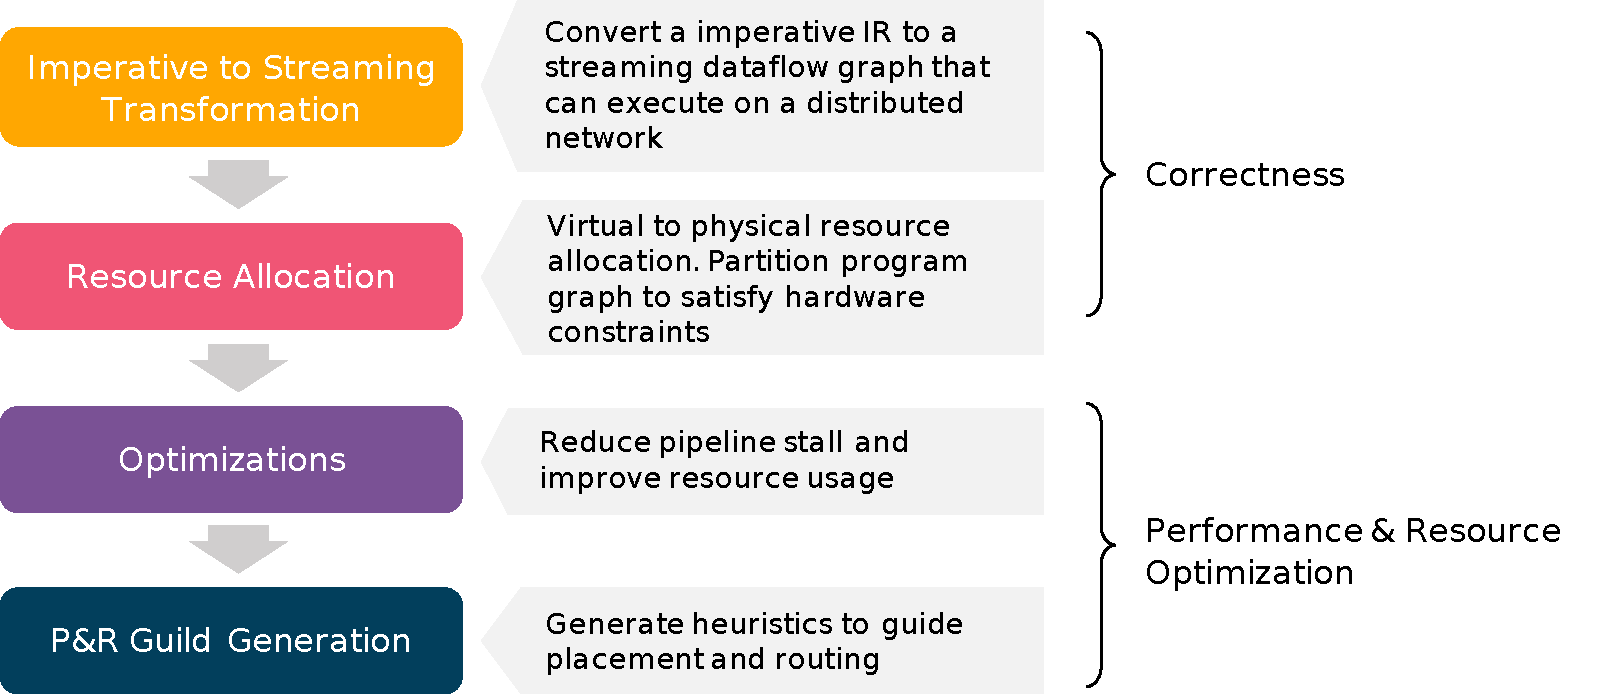
\includegraphics[width=1\textwidth]{figs/sarastack.pdf}
\caption[\name Compiler Flow]{\name Compiler Flow}
\label{fig:flow}
\end{figure*}
 
In this section, we describe a systematic approach to compile applications described in an
imperative front-end language with into a purely declarative and distributed dataflow graph that can
run on Plasticine.
\Cref{fig:flow} shows the compilation flow to perform this translation between the two paradigms.
At high-level, \name allocates distributed on-chip resources to execute the program in spatially parallelized and
pipelined fashion.
\name automatically generates synchronization across distributed units to provide strong 
memory consistency for a imperative program, on an architecture that does not guarantee memory
ordering across multiple access streams.
This synchronization is purely point-to-point that introduces minimum performance overhead, which
maximizes scalability of the architecture.
\name further virtualizes resources allocation and hides the underlying resource constrains on
this hierarchical architecture from the programmers.

First, \name takes the input Spatial IR and performs the \term{virtual allocation}.
A virtual unit (VU) is our intermediate representation that captures computations that will be
mapped onto a physical unit (PB), such as a PCU and PMU.
The compiler can allocate multiple contexts within a virtual unit. However, messages across 
VUs must tolerate arbitrary amount of network latencies, whereas messages across contexts within a single VB
takes a single cycle.
In this phase, \name generates p2p message passing as if there are centrolized scheduler scheduling
the execution at each level of the nested control hierarchy in the original program.
The allocation phase generates a virtual unit data-flow graph (VUDFG) with appropriate
synchronizations, such that the on-chip distributed execution produces the same result as if the program is
sequentially executed.

At the end of the allocation phase, a virtual unit can consume as much resource as the program
requires. The second phase is \term{physical allocation}, where \name assign each VU to a
PU that processes the required resources. If no PU can execute a VU, \name tries to partition the
VU into multiple VUs to eliminate constraint violation. If there is insufficient PU or the
VU cannot be partitioned, the mapping process fails.

Throughout the first two phases, \name introduces various \term{optimizations} that either reduce the
resource cost of the VUDFG, or alleviates potential performance bottleneck in streaming pipelined execution.
After all VU fits in at least one type of PU, \name performs a global optimization that merges 
small VUs into a larger VU to reduce resource fragmentation.

At the end the previous phase, each VB is tagged with a PB type that can fit the VB, and it is up to the
\term{placement and routing (PaR)} phase to determine where the VB will be finally placed.
\name can perform static analysis on the communication traffic and generate heuristics for PaR to
reduce runtime congestion.

In the following sections, \Cref{sec:control} describes conversion from imperative paradigm with
nested control hierarchy to the distributed streaming data-flow execution.
\Cref{sec:decompose} details program-partitioning passes that decompose program over distributed resources.
\Cref{sec:opt} enumerates several optimizations in \name, and \Cref{sec:par} discuss about PaR and
heuristic generation.

\begin{figure*}
\centering
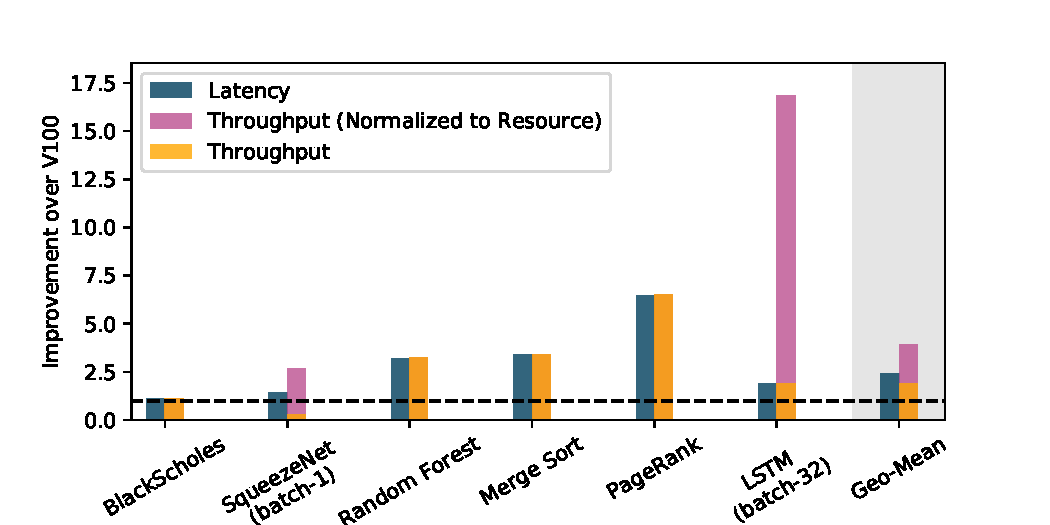
\includegraphics[width=1\textwidth]{figs/slide_gpu.pdf}
\caption[Performance comparison with V100 GPU]{
  Plasticine's latency and throughout improvement over V100 GPU.
  The evaluated Plasticine architecture has area footprint of 352$mm^2$ at 28nm.
  V100 GPU has area footprint of 815$mm^2$ at 12nm.
  Both platforms have the same off-chip bandwidth at 1TB/s with HBM technology.
  Yellow and blue bars show the raw measured speedup in throughput and latency, respectively.
  To account for the resource discrepancy, the pink bar shows the normalized throughput
  for compute-bound application--SqueezeNet and LSTM, which scales performance with additionally
  on-chip resources.
}
\label{fig:peakutil}
\end{figure*}
